\section{Introduction}

Unmanned aerial vehicles capable of vertical takeoff and landing have undergone a big boom in past few years. It is mainly thanks to arrival of multirotor helicopters (multicopters). Their capabilities span from being a platform for professional film makers, to toys and hobby products, up to military vehicles built for reconnaissance. These vehicles (fig. \ref{fig:quadru1}) have characteristically several propellers (typically four and more) with fixed pitch angle. The machine itself is usually a simple design by comparison with a classical helicopter. From the mechanical point of view it has several brushless motors with propellers mounted directly on them. There is a rigid body with utility platform, motor mounts and landing gear. They can operate in situations where the presence of a person could be hazardous (natural disasters) or they can help with work tasks which would otherwise require a very expensive solution e.g. control of high-voltage lines. They find an application in situations where prior technology would not help --- archaeological imaging from low-to-mid altitude.

In most cases such aircraft requires a human operator to fly although it can offer a certain level of automatic assistance. Nowadays the global position system (GPS) is embedded literally in every mobile phone thus it is no surprise that it can help with control of an unmanned aircraft (UAV) when flying outdoors. Commercially available platforms can assist with position hold or even flight to a particular location. Such technology can provide an automatic flight with precision up to $1 \jed{m}$ depending on GPS, external conditions and the vehicle itself. The scientific community showed that there are methods to increase the precision of UAV control up to centimeters by using a better localization system then GPS (namely Vicon system) and implementing advanced algorithms for automatic control \citep{brescianini2013polearobatics, kumar2010grasp}.

\begin{figure}[h]
\centering
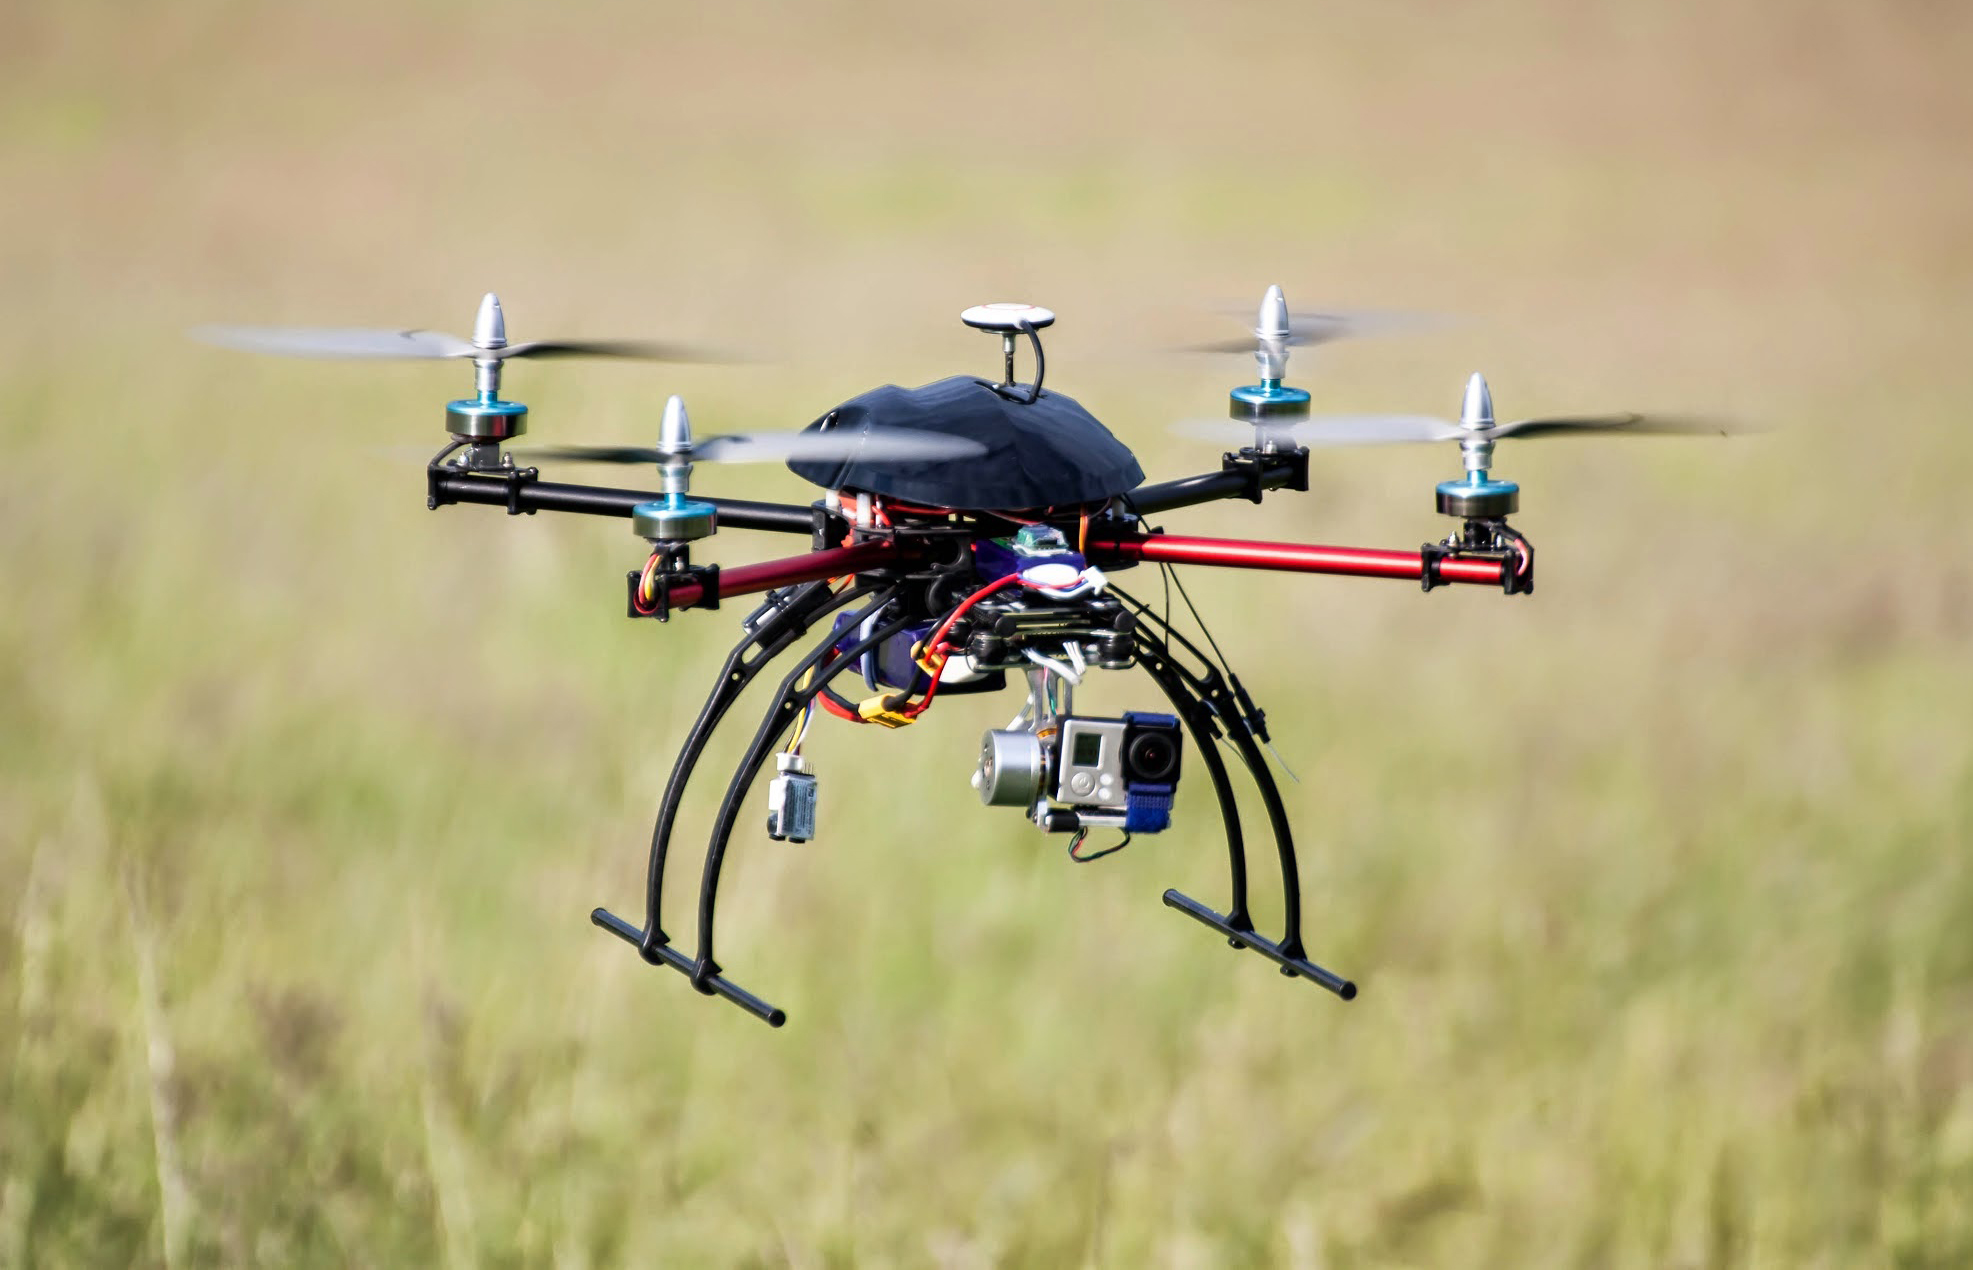
\includegraphics[width=0.8\textwidth]{fig/quadru1.jpg}
\caption{An example of multirotor aircraft used for aerial imaging.}
\label{fig:quadru1}
\end{figure}

Although previously mentioned work required an expensive laboratory hardware and on the ground computational power, it can be used as an example of what one could imagine an ''automatic assistance'' would be capable of when flying indoors. Since the multirotor UAV is a highly unstable machine (it will fly away when not controlled) there is feedback control necessary to even stop it in the air. UAVs have been a subject of research for a long time. There is a current one with intention to build an automatic UAV that is supposed to work not only in a laboratory but also in uncontrolled indoor environment. That may seem as a modification of current outdoor solutions but in practice it brings in new challenges and requires different approaches. The main ones are requirement of high precision control when flying indoors while omitting external localization system (like Vicon and GPS) and managing all computations onboard the vehicle itself.

The control mechanism used in today control systems is usually satisfactory when the precision is roughly defined by the GPS localization and the control settling time is slow. It is often narrowed to PID (proportional-integral-derivative controller) that is relatively easy to compute on common embedded hardware \cite{pixhawk, ardupilot}. But when increasing requirements on precision and settling time, such approach seems to suffer when controlling this kind of unstable vehicle (see prior work in chapter \ref{cap:prior_work}). Also when imposing a requirement not to only stabilize the vehicle (stop it from movement) but to fly through a desired space trajectory, the need for a better control design approach emerges.

\subsection{Problem statement}

\subsection{Related work}

\subsection{Previous work}
\label{cap:prior_work}

\subsection{Contribution}